
\subsection{Locating Errors with Witnesses}
\label{sec:locating}

We have seen that \toolname can effectively synthesize witnesses to
explain the majority of (novice) type errors, but a good error report
should also help \emph{locate} the source of the error.
%
Thus, our final experiment seeks to use \toolname's witnesses as
localizations.


As discussed at the beginning of \S~\ref{sec:evaluation}, we recorded
each interaction of our students with the \ocaml top-level system.
%
In addition to collecting ill-typed programs, we collected
subsequent, fixed versions of the programs.
%
We identify fixed programs by searching for the first type-correct
program that follows the ill-typed program in the interaction trace.
%
We then use an expression-level \emph{diff}~\cite{Lempsink2009-xf} to
determine which sub-expressions changed between the ill-typed program
and the student's fix, and treat those expressions as the source of the
type error.

Not all ill-typed programs will have an associated fix; furthermore,
at some point a ``fix'' becomes a ``rewrite''.
%
We do not wish to consider the ``rewrites'', so we discard outliers
where the fraction of expressions that have changed is more than one
standard deviation above the mean, establishing a diff threshold of
45\%.
%
This accounts for roughly 14\% of programs pairs we discovered, leaving
us with 2,425 program pairs.

For each pair of an ill-typed program and its fix, we run \toolname and
collect two sets of source locations:
%
(1) the source location corresponding to the stuck term; and
%
(2) the source locations that \emph{produced} the values inside the
stuck term.
%
Intuitively, these two classes of locations correspond to \emph{sinks}
and \emph{sources} for typing constraints.
%
For example, in the @sqsum@ program from \S~\ref{sec:advantage-traces}
the stuck term is \verb!0 @ 1!.
%
This corresponds to the call to \verb!@! on line 3, and contains
the literal @0@ from line 2 and the value @1@ produced by the
@*@ on line 3.

We compare \toolname's witness-based predictions against a baseline of
the \ocaml compiler as well as the state-of-the-art tools \sherrloc
and \mycroft.
%
\sherrloc attempts to predict the most likely source of a type error
by searching the typing constraint graph for constraints that participate
in many unsatisfiable paths and few satisfiable paths.
%
\mycroft reduces the localization problem to MaxSAT by searching for a
minimal subset of constraints that can be removed, such that the
resulting system is satisfiable.
%
Both tools produce a \emph{set} of equally-likely expressions to blame
for the error (in practice the set contains only a few expressions),
similar to \toolname's witness-based predictions.

We evaluate each tool based on whether \emph{any} of its predictions
identifies a changed expression.
%
There were a number of student programs where \mycroft or \sherrloc
encountered an unsupported language feature or timed out after one
minute, or where \toolname failed to produce a witness.
%
We discard all such programs in our evaluation to level the playing
field, leaving us with a benchmark set of 1,612 programs.

\begin{figure}[t]
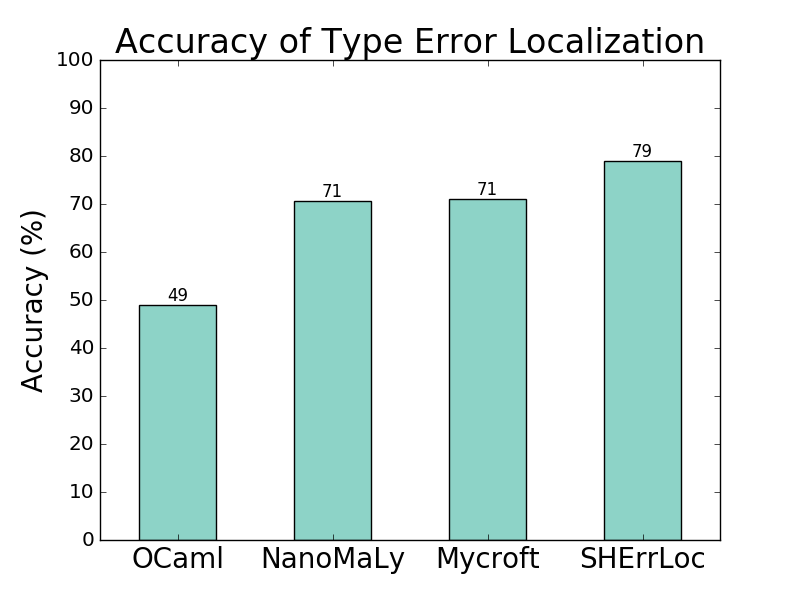
\includegraphics[width=0.8\linewidth]{blame.png}
\caption{Accuracy of type error localization. \toolname's witness-based
  predictions outperform \ocaml by 20 points, and are competitive
  with the state-of-the-art tools \mycroft and \sherrloc.}
\label{fig:results-blame}
\end{figure}

\paragraph{Results}
Figure~\ref{fig:results-blame} summarizes our results, which show that
\toolname's witnesses are competitive with \mycroft and \sherrloc in
automatically locating the source of a type error.
%
\toolname, \mycroft, and \sherrloc all outperform the \ocaml compiler,
which is not surprising given that they can produce multiple possible
error locations, while the \ocaml compiler is limited to one predicted
error location.
%
Interestingly, while all tools have a median of 2 predicted error
locations per program, \mycroft and \sherrloc have a long tail with a
maximum of 22 (\resp 12) locations, while \toolname's maximum is 5
locations.
%
We also note that while \mycroft and \sherrloc were designed
specifically to \emph{localize} type errors, \toolname's foremost
purpose is to \emph{explain} them, we consider its ability to localize
type errors an added benefit.

%%% Local Variables:
%%% mode: latex
%%% TeX-master: "main"
%%% End:
